\chapter{Player Agents}
In order to test our networks we designed baseline agents to play against, to measure playing strength.
The agents all use same \textit{makebid()} method to establish an even playing field, on which we can compare pure
playing strength.
Each agent's strategy will be briefly explained and statistics from a fair tournament, whicht is playe between four
instances of the respective player,will be given to get an idea.


\section{Static Bidding}
Table \ref{tab:distributionBidding} shows the distribution of contracts.
We can see that the majority of hands are Team contracts, whilst the remaining 15\% of games are envenly distributed
over the remaining Solo contracts.\\
The bidding heuristic used here is by no means expert play but overall reasonable for what we are trying to achieve.
Human players are likely to play a somewhat higher percentage of Solo games, although that frequency is heavily
affected of one's one playing strength, and ideally varied according to one's opponents abilities.
To find a balance between win rate and winning frequency is major part in contract card games such as Bridge and
Schafkopf.
\begin{table}[!h]
    \centering
    \begin{tabular}{lc}
        \toprule
        Contract    & Distribution \\
        \midrule
        Team        & 85,3         \\
        Wenz        & 6,6          \\
        Colour-Solo & 8,1          \\
        No Game     & 0,0          \\
        \bottomrule
    \end{tabular}
    \caption{Distribution of contracts}
    \label{tab:distributionBidding}
\end{table}


\section{Baseline Agents}

\subsection{Random Agent}
The Random agent plays like the name suggests a random valid card.
It makes no use of the passed games state, has no understanding of team composition and performs expectantly bad.
This strategy is terrible for all contracts, although some hands can still be played near optimal, due to holding good
cards, having competent teammates, or having little choice.
\begin{table}[!h]
    \centering
    \begin{tabular}{ccccccc}
        \toprule
        Team  & Wenz  & Solo  & Team-Partner & Sauspiel-Opp & Wenz-Opp & Solo-Opp \\
        \midrule
        0.616 & 0.539 & 0.843 & 0.616        & 0.384        & 0.461    & 0.157    \\
        \bottomrule
    \end{tabular}
    \caption{Average win rates of Random agent against itself over 10000 hands}
    \label{tab:winratesRan}
\end{table}

\subsection{Greedy Agent}
The Greedy agent will always try to win every trick possible.
It understands trumps, tricking, point values, but has no understanding of team composition.
When he has the lead it chooses to play the highest rank that is not trump, or the highest trump if it only holds trump.
When not in the lead it will test if it can beat the cards in the current trick, even if one of his partner currently
is the trick winner.
If it holds more than one winning card it will choose the card with the highest point value.
Vice Versa if it holds no winning card it will choose the lowest point value card, if possible not trump, even if
that means playing an Ace.\\
In summary,Greedy agent values winning tricks and not giving up trump if possible.
This strategy can certainly be viable for Solo contracts where itself is the bid winner, but will fail when it is
part of the opposition, because trumps are sparse and over-tricking teammates is major error.
For team contracts it [LOOK at stats, might be ok for]
\begin{table}[!h]
    \centering
    \begin{tabular}{ccccccc}
        \toprule
        Team  & Wenz  & Solo  & Team-Partner & Sauspiel-Opp & Wenz-Opp & Solo-Opp \\
        \midrule
        0.604 & 0.646 & 0.757 & 0.604        & 0.396        & 0.354    & 0.243    \\
        \bottomrule
    \end{tabular}
    \caption{Average win rates of Greedy agent against itself over 10000 hands}
    \label{tab:winratesGre}
\end{table}

\subsection{Heuristic Agent}
The Heuristic agent is a lot more nuanced than the above agents.
It employs a separate strategy for each of seven game positions and uses the game state to infer the team composition
,if possible, and uses the strategies from \ref{basicstrategy} to some extent.\\
Furthermore it understands everything Greedy agent knows, about points, trump and tricking.
Its limitations are its use of the trick history, which is only used when it plays in the offensive or team partner
role to infer how many trumps are still with the others, but misses strategies, such as leading a suit where a
teammate is known to be, or similar.
The decision process is mostly deterministic, but there are situations where two cards are equally playable and one is
randomly chosen.\\
Heuristic agent is certainly a decent opponent that follows good practice play a novice might bring to the table.
[FLOWCHART]
\begin{table}[!h]
    \centering
    \begin{tabular}{ccccccc}
        \toprule
        Team  & Wenz  & Solo  & Team-Partner & Sauspiel-Opp & Wenz-Opp & Solo-Opp \\
        \midrule
        0.485 & 0.588 & 0.695 & 0.485        & 0.515        & 0.412    & 0.305    \\
        \bottomrule
    \end{tabular}
    \caption{Average win rates of Heuristic agent against itself over 10000 hands}
    \label{tab:win ratesHeu}
\end{table}


\section{Reinforcement Learning Agents}
The models we trained are simple {\textbf{feed forward NN} that receive a game state, which is processed and then fed
through the Network to produce two outputs: 32x1 vector that gives us our probabilities of all the valid
actions (\textit{actor}), and 1x1 vector which describes our state-value function (\textit{critic}). (See Fig
.\ref{fig:layerchart})\\
All inner layers use 48 hidden \textbf{ReLÚ} neurons
Overall we trained two agents, \textbf{CompleteRL} and \textbf{SeperatedRL}, that both use the same actor-critc network
design.
\begin{figure}[!h]
    \centering
    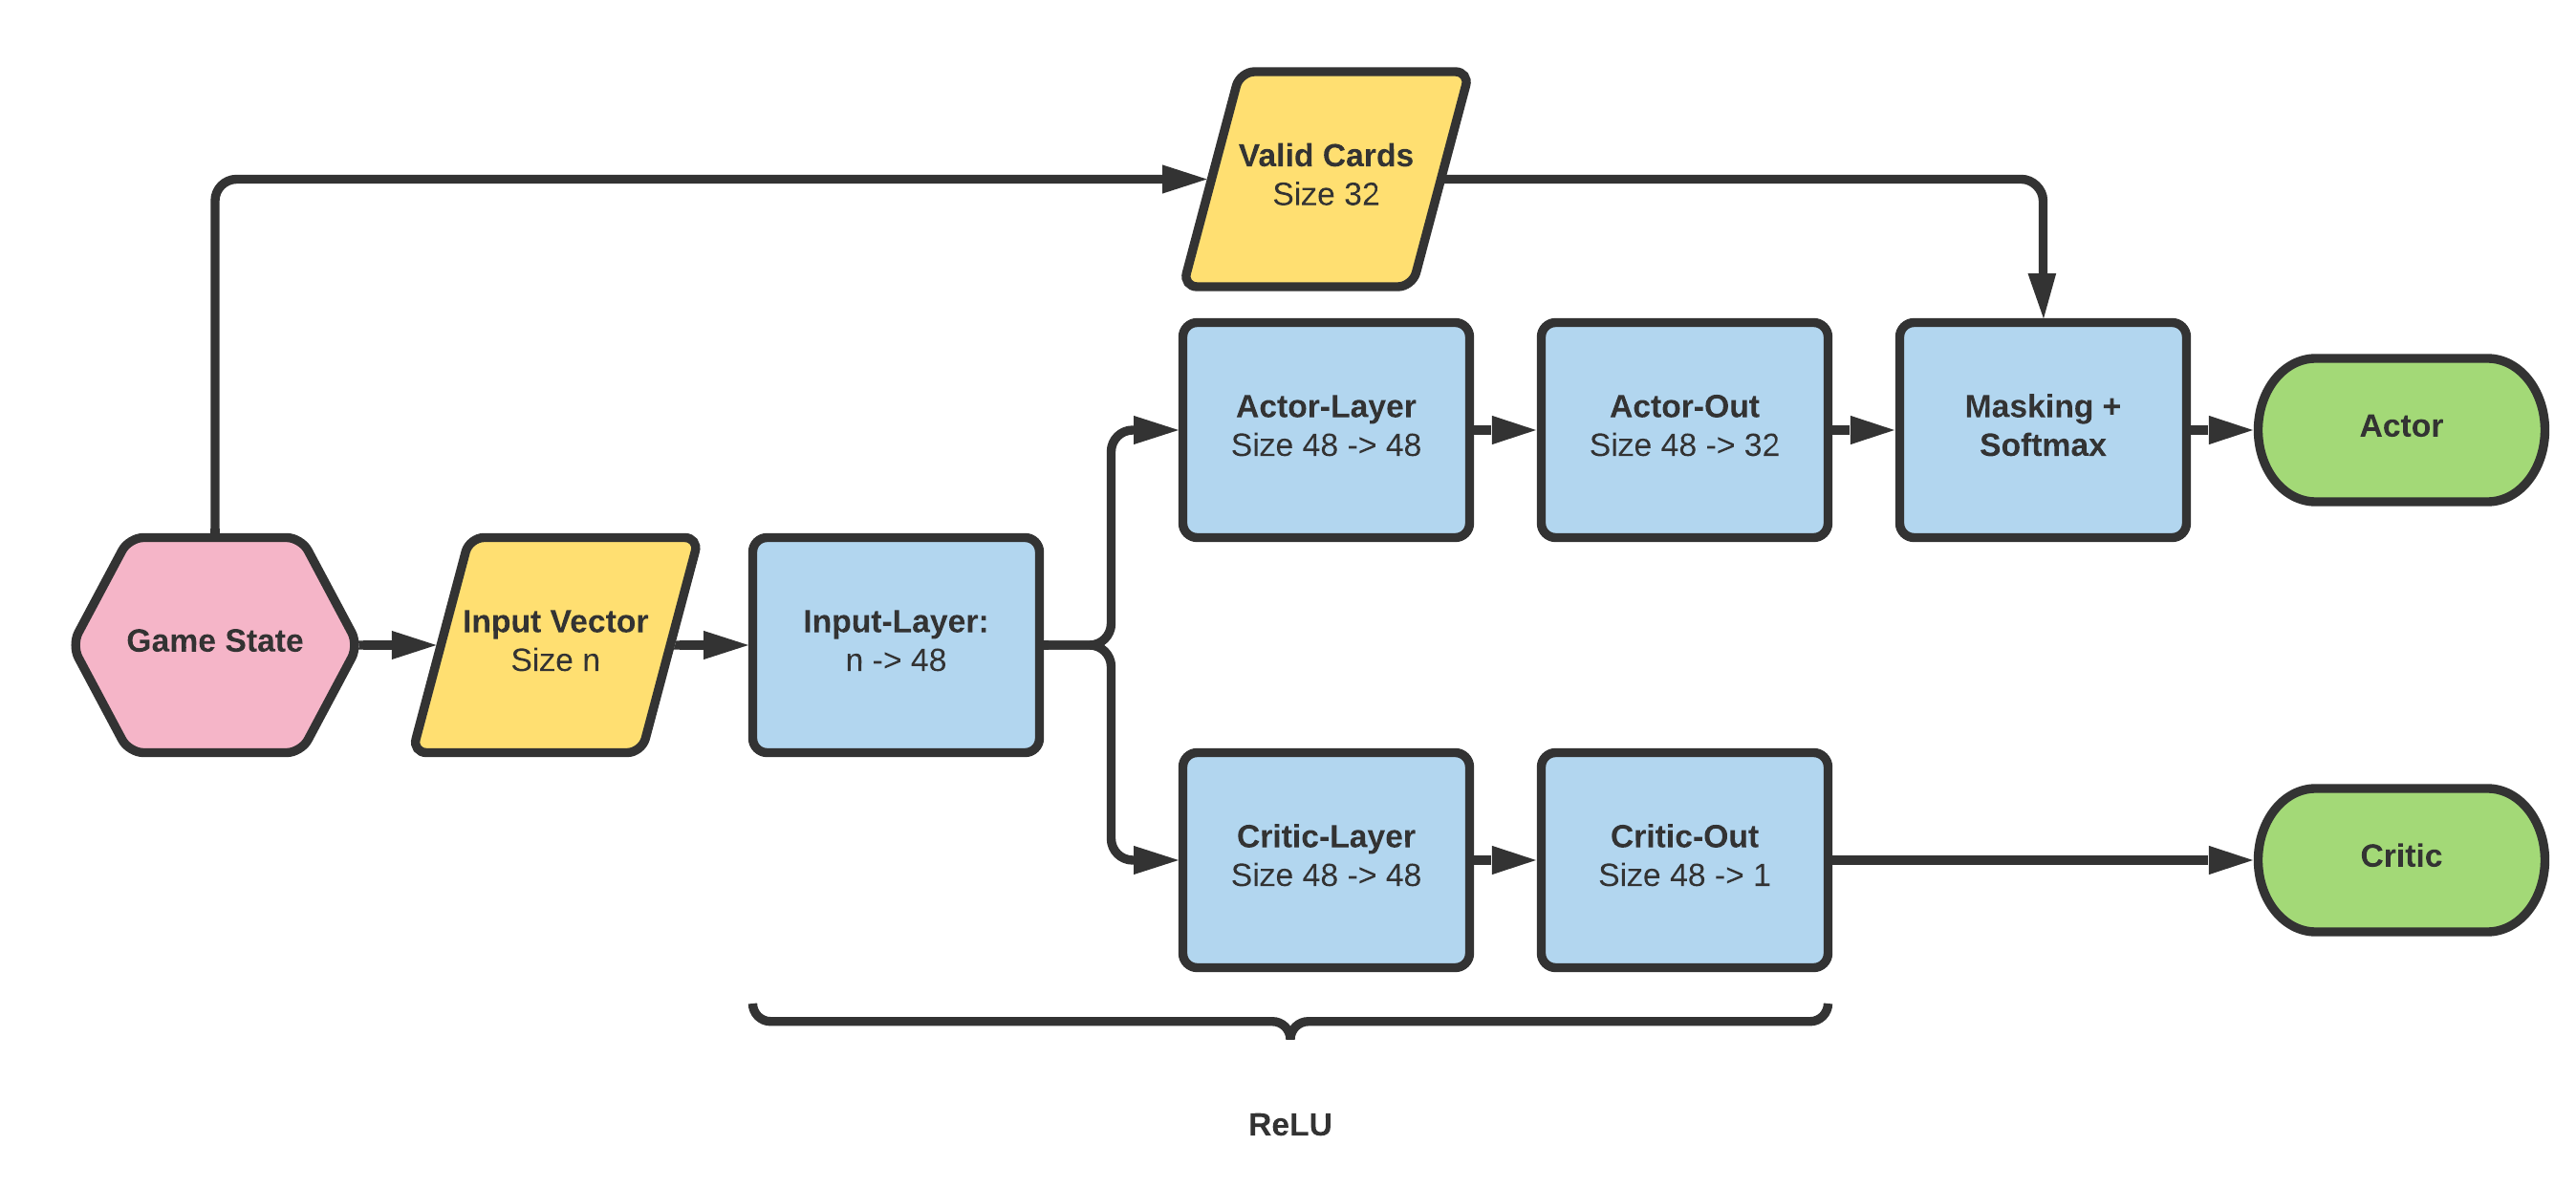
\includegraphics[width=\textwidth]{layerchart.png}
    \caption{Network layer flow used the Actor-Critic Models}
    \label{fig:layerchart}
\end{figure}
\end{center}
\subsubsection{CompleteRL}
The CompleteRL agent uses the same network for all three game modes.
This was our initial approach, to see if one network can do it all.
The input vector (See Tab. \ref{tab:CompleteRLinput}), derived from the game state, uses \textit{one hot encoding}
for all cards, positions and information and is always rotated so the acting player is in position zero, to keep the
vector representation
consistent.\\
\begin{table}[!h]
\centering
\begin{tabular}{lll}
\toprule
Name          & Size     & Description                                           \\
\midrule
Hand          & 32       & Hand of the player                                    \\
Cards Played  & 32       & All cards in previous tricks                          \\
Lead          & 4        & Position that started the trick                       \\
Game Mode     & 7        & 3 contracts + 4 colours                               \\
Ran Away      & 1        & If partner ran away (Bool)                            \\
Searched      & 1        & If the ace has been searched (Bool)                   \\
Bid Winner    & 4        & Position that won the bidding                         \\
Own Team      & 4        & Position of own Team (1000 if unknown)                \\
Scores        & 4*1      & Scores for each position (Normalised using Score/120) \\
Trick History & (32+4)*4 & Cards played by each position                        \\
\midrule
Sum & 233 & Total size of the input Vector\\
\bottomrule
\end{tabular}
\caption{Input vector for the CompleteRL model}
\label{tab:CompleteRLinput}
\end{table}

\subsubsection{SeperatedRL}
As an experiment we also trained \textbf{SeperatedRL} that has a different model for each of the three contracts
(Team,Wenz,Solo).
The idea is to reduce the variance in the training data, whilst also only including the relevant information and thus
slimming the input vector.
The major drawback of this is naturally training time, but we reduced the batch size during training compared to
\textbf{SeperatedRL} but tried to keep learning steps when evaluation the two.

\begin{table}[!h]
\centering
\begin{tabular}{lllll}
\toprule
Name          & \multicolumn{3}{c}{Size}                                               & Description
\\
\midrule
& Team     & Wenz                      & Colour-Solo                     &
\\
\midrule
Hand          & 32       & 32                        & 32                              & Hand of the player
\\
Cards Played  & 32       & 32                        & 32                              & All cards in previous tricks
\\
Lead          & 4        & 4                         & 4                               & Position that started the
trick                       \\
Game Mode     & 4        & 0 & 4                               & 4 colours
\\
Ran Away      & 1        & 0 & 0       & If partner ran away (Bool)                            \\
Searched      & 1        & 0 & 0       & If the ace has been searched (Bool)                   \\
Bid Winner    & 4        & 4                         & 4                               & Position that won the
bidding                         \\
Own Team      & 4        & 4                         & 4                               & Position of own Team (1000
if unknown)                \\
Scores        & 4*1      & 4*1                       & 4*1                             & Scores for each position
(Normalised) \\
Trick History & (32+4)*4 & (32+4)*4                  & (32+4)*4} & Cards played by each position
\\
\midrule
Sum           & 214      & 208                       & 212                             & Total size of the input
Vector\\
\bottomrule
\end{tabular}
\caption{Input vector for each sub model of the SeperateRL agent}
\label{tab:Seperatedinput}
\end{table}

